\chapter{Verification of confirmations}

\section{Network Model}

We assume a multihop network with a set $ S = \{s1,...,s_{n}\} $ of $n$
sensor nodes. The network is organized in a tree topology, with the
base station as the root of the tree. The trusted querier resides
outside of the network \& has more computation, storage capacity 
then the sensor nodes in the network. The base station and the 
querier knows total number of sensor nodes $n$ and the network 
topology. All the wireless comuunication is peer-to-peer and we do 
not consider local wireless broadcast. We also assume that the
querier has the capacity to do peer to peer communication with 
every sensor node in the network. We also assume that all the sensor nodes 
mapped to the vertices in the commitment tree who reported the authentication 
codes with NACK messages during the collection of confirmations step are 
honest. 

\subsection{Sensor Nodes}

	We assume that each sensor node has a unique identifier $s$ and
	shares a unique secret symmetric key $K_{s}$ with the querier. 
	We assume all the sensor nodes are capable of doing symmetric-
	key encryption and symmetric key decryption. They are also
	capable of computing collision-resistant cryptographic hash 
	function $H$. We also assume that if the sensor node has to send 
	multiple messages to its parent it can combine those messages 
	into single packet in a way that parent node can distinguish both 
	the messages.

\subsection{Commitment trees} % (fold)
\label{sub:Commitment trees}
		
	The aggregation tree is a physical network over which all the
	communication happens while the commitment tree is a logical
	network on top of aggregation tree. In the similar manner, 
	vertices in a commitment tree is a logical element in a graph 
	while a sensor node is a physical device. 

	The commitment trees have the following properties. 
	At most there will be $\lceil lg  n \rceil$ commitment trees in the forest for an aggregation tree with $n$ sensor nodes.
	The binary representation of the number of sensor nodes $n$ in the network indicates the number of commitment trees in the forest. It also indicates the height of all the commitment trees in the forest. 
	For instance, if there are $ 11_{10} = 1011_{2} $ sensor nodes in the aggregation tree then there will be three commitment trees in the forest. From those three commitment trees, one will be of height three, one will be of height one and one will be of height zero.
	At most there will be $n + ( n - 1 )$ vertices in the forest of commitment trees for an aggregation tree with $n$ sensor 
	nodes.

	\textit{It is also possible that only one sensor node $s$ in the aggregation tree, will be the root vertex of all the commitment trees in the forest.} 

	\textit{It is also poosible that all the internal vetices in the commitment tree are of different sensor nodes in the aggregation tree.}


% subsection Commitment trees (end)

\subsection{Collections of confirmations}
After each sensor node $s$ has successfully performed the 
verification step for its leaf vertex $u_{s}$, it sends an 
authentication code to its parent in the aggregation tree.
The authentication code for sensor node $s$ is MAC$_{K_{s}}(N||ACK)$
where ACK is an acknowledgemnet message, N is the query nounce and $K_{s}$ 
is the secret key that sensor node $s$ shares with the trusted querier. Once
an internal sensor node $s$ in the aggregation tree has received the
authentication codes from all of its descendants, it computes the XOR of its 
own authentication code with all the received authentication codes, and 
forwards the result to its parent. Finally, the querier will receive a 
single authentication code from the base station that consists of the XOR of 
all the authentication codes received in the network. 

\subsection{Verification of confirmations}
Since the querier knows the secret key $K_{s}$ for each sensor node $s$ in the aggregation tree and it also knows the topology of the commitment trees in the forest, it can simulate the commitment trees in the forest. The querier simulates the commitment trees in the forest by computing the following authentication codes\\

MAC$_{K_{1}}(N||ACK)\,\oplus\,$ 
MAC$_{K_{2}}(N||ACK)\,\oplus\,$
...
$\,\oplus\,$
MAC$_{K_{n}}(N||ACK)$ ; \\
MAC$_{K_{1}}(N||NACK)\,\oplus\,$ 
MAC$_{K_{2}}(N||NACK)\,\oplus\,$
...
$\,\oplus\,$
MAC$_{K_{n}}(N||NACK)$  \\


and creates two simulated commitment trees, one with the authentication codes of ACK messages and one with the authentication codes of NACK messages; where ACK is an acknowledgemnet message, NACK is a negative acknowledgemnet message \& N is the query nounce. Then the querier merges all the commitment trees in the forest simulated with the authentication codes of ACK messages, by taking XOR of the root of all the commitment trees in the forest and calculates a single root authentication code for the forest simulated with the authentication codes of ACK messages. The querier does the same procedure for the commitment trees' forest simulated with the authentication codes of NACK messages. The querier stores all the simulated commitment trees and root authentication codes in the memory. \\


The querier receives a signle root authentication code from the base station during the collection of confirmation messages step. The querier compares the received root authentication code with the relevant simulated authentication code of ACK messages. If those two codes match it means every vertices in the subtree rooted at that vertex sent the authentication codes with ACK message during collection of confirmation step. If those two codes do not match it means one or more vertices in the subtree rooted at that vertex sent the authentication codes with NACK message during collection of confirmation step. In the case where root authentication codes do not match, the querier proceeds futher to find out which vertex or vertices in the network sent the authentication codes with NACK message during collection of confirmation messages step.\\


To find out which vertex or vertices in the commitment tree reported the authentication codes with NACK message, the querier asks the base station to send the authentication codes of all the commitment trees' root in the forest. After receiving the authentication codes from the base station, the querier compares those authentication codes with the relevant simulated authentication codes of ACK messages. After this comparision, whose authentication codes do not match, the querier classifies those commitment trees as BAD TREES in the forest. \\


Then the querier compares the authentication codes of those BAD TREES with the relevant simulated authentication codes of NACK messages. If any of those authentication codes match it means all the vertices rooted in that subtree sent the authentication codes with NACK message during the collection of confirmation stpe. And the querier stops doing the quiers to the subtree rooted at that vertex. If those authentication codes do not match then the querier proceeds furhter to find the senosr node or nodes who reported the authentication codes with NACK message in BAD TREES.\\


\subsection{Algorithm for detecting vertex or vertices who reported authenctication codes with NACK messages }

For each BAD TREE in the forest the querier does the following :

\begin{enumerate}
 
   \item 
  The querier asks the relevant nodes in the aggregation tree to send the authentication codes of their children in the commitment trees.

  \item
  The querier compares the received authentication codes in step 1 with the authentication codes of the relavant vertices of the commitment trees simulated with the authentication codes of ACK messages. The querier classifies the subtree rooted at those vertices as BAD SUBTREES, whose authentication codes do not match.

  \item 
  The querier compares the received authentication codes in step 1 with the authentication codes of the relavant vertices of the commitment trees simulated with the authentication codes of NACK messages. If those codes match it means all the vertices rooted in that subtree reported NACK messages during collection of confirmation steps. And the querier stops doing the queries to that subtree. If those codes do not match then the querier goes to step 2. \\

  The querier follows this algorithm until it finds all the vertices who reported the authentication codes with NACK messages in the commitment trees during collection of confirmation step.

\end{enumerate}




\subsection{Analysis} % (fold)
\label{sub:analysis}

To simulate the commitment trees in the forest the querier has to do the following calculations. Suppose there are $n$ sensor nodes in the network, means there will be at most $\lceil lg n \rceil$ commitment trees in the forest. If there are $n^{'}$ leaves in each commitment tree in the forest then the height($h^{'}$) of each commitment tree will be $lg(n^{'})$ and the number of intermediate vertices ($i^{'}$) in the network will be ($ 2^{h^{'}} - 1 $). So, there will be total of  $ (n^{'} + i^{'}) $ * $\lceil lg  n \rceil $  vertices in the forest. As the querier needs to simulate two commitment trees one for ACK messages and one for NACK messages it has to do ( $ 2 * (n^{'} + i^{'}) * \lceil lg  n \rceil $ ) calculations.

As we know from the properties of commitment trees, at most there 
will be $n + ( n - 1 )$ vertices in the forest of commitment trees 
for an aggregation tree with $n$ sensor nodes. So, the querier has
to do $ 2 * ( n + ( n - 1 ) )$ calculations and it also need that much memory space to store those values.

With Dr.King with a single NACK message in a tree:

Maximum number of leaves in a single commitment tree is equal to $n$. 
So, we can upper bound it with $O(n)$. As there is a signle NACK 
message in the tree, during verification phase we know in which part 
that vertex is. 

So, we can identify the node in at most $\log{n}$ steps.
We need $2*\log{n}$ messages to identify that. The querir will have to 
ask $\log{n}$ times and some node from the aggregation time has to 
reply $\log{n}$ times. This is total number of messages is required but 
number of communication depends on the aggregation tree.

Worst case:
In the worst case, the querier has to ask values of all the vertices in 
the commitment tree. At max there will be $(2*n - 1)$ messages. Again, 
remember these are the number of messages, number of communications 
might be different.

Best case in terms of number of communications:
It needs minimum number of communications when one single node is
everywhere in the aggregation tree. In that case if the querier has to 
know the values of all the leaves vertices it has to ask $\log(n)$ 
questions and node has to reply to those messages. So, number of 
communication is equal to $2 *log(n)$.


% subsection analysis (end)

\begin{figure}[t]
	\centering
		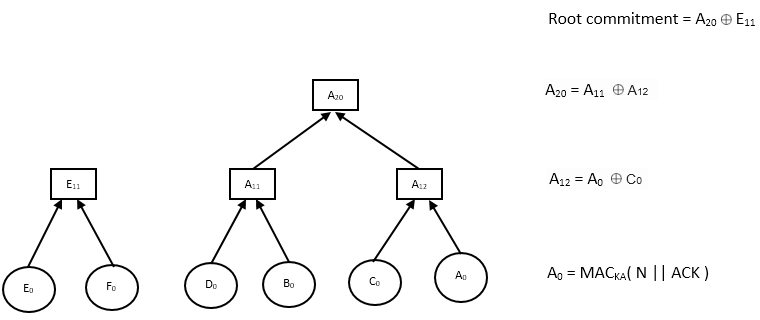
\includegraphics[width=0.8\textwidth]{ack.png}\\
		\caption{Simulated commitment tree with ACK messages}
	\label{fig:figure1}
\end{figure}

\begin{figure}[t]
	\centering
		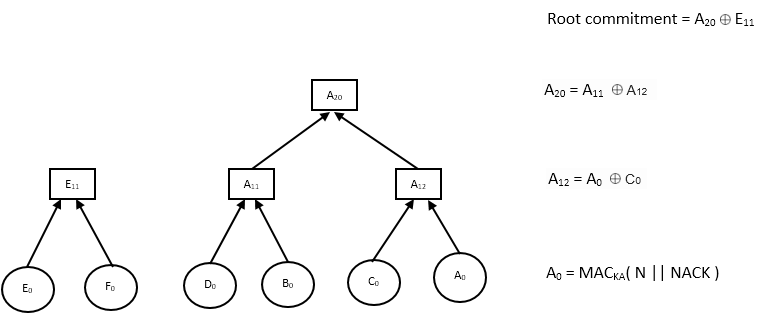
\includegraphics[width=0.8\textwidth]{nack.png}\\
		\caption[Simulated commitment tree with NACK messages]{Simulated commitment tree with NACK messages}
	\label{fig:figure1}
\end{figure}

